% StudyOS Thesis-Finder — faculty presentation
% Build: latexmk -pdf studyos-thesis-finder.tex
\documentclass[11pt,aspectratio=169]{beamer}

\usetheme[progressbar=frametitle]{metropolis}
\usepackage[T1]{fontenc}
\usepackage[utf8]{inputenc}
\usepackage{booktabs}
\usepackage{tikz}
\usetikzlibrary{arrows.meta,positioning,shapes.misc}

% Slightly calmer metropolis accents
\definecolor{sosAccent}{HTML}{2A6F77}
\definecolor{sosDark}{HTML}{23373B}
\setbeamercolor{progress bar}{fg=sosAccent}
\setbeamercolor{frametitle}{bg=sosDark}
\setbeamercolor{alerted text}{fg=sosAccent}

\newcommand{\quotebox}[1]{%
  \begin{beamercolorbox}[rounded=true,sep=0.6em]{block body}%
    \itshape #1%
  \end{beamercolorbox}}

\title{StudyOS Thesis-Finder}
\subtitle{Better-prepared students, fewer misdirected inquiries}
\author{StudyOS Team}
\institute{Department of Computer Science, University of Tübingen}
\date{July 2026}

\begin{document}

\maketitle

\begin{frame}{The problem, from both sides}
  \begin{columns}[T]
    \begin{column}{0.48\textwidth}
      \textbf{Students}
      \begin{itemize}
        \item Spend weeks figuring out which chairs even work on their interests
        \item See 4--5 listed topics, assume that is the whole lab, and never reach out
        \item Send generic cold emails to the wrong chairs
      \end{itemize}
    \end{column}
    \begin{column}{0.48\textwidth}
      \textbf{Professors}
      \begin{itemize}
        \item Receive far more inquiries than they can supervise \\ (one chair: 50+ inquiries for 20 slots)
        \item Spend time writing rejections they regret
        \item Get low-signal first contacts that miss the chair's actual research
      \end{itemize}
    \end{column}
  \end{columns}
  \vspace{1em}
  \begin{center}
    \alert{Both sides lose to the same failure: low-signal first contact.}
  \end{center}
\end{frame}

\begin{frame}{What 27 professors in this department told us}
  We interviewed 27 professors before building anything. The verdict on a
  classic \emph{topic-listing platform}:
  \begin{itemize}
    \item \textbf{$\sim$50\%} do not want a central platform --- either already
      overrun with applicants, or convinced topics must be
      \emph{co-created in conversation}, not browsed from a list
    \item \textbf{$\sim$35\%} would try a tool --- but only if zero-friction,
      with no reminder emails, and stable for years
    \item \textbf{$\sim$15\%} recruit through other channels entirely
  \end{itemize}
  \quotebox{``Profs never update the topics. We've had many attempts in the
  department already.''}

  A topic platform was tried here around 2022 and failed --- for
  \alert{incentive} reasons, not UI reasons.
\end{frame}

\begin{frame}{Our conclusion: build for students, not for chairs}
  \begin{center}
    \large A tool that requires \alert{zero professor participation} to deliver value.
  \end{center}
  \vspace{0.4em}
  The agent helps a student to:
  \begin{enumerate}
    \item \textbf{Formulate} --- turn vague interests, coursework, and skills
      into a structured competency profile
    \item \textbf{Discover} --- find which chairs and researchers actually work
      on relevant problems, based on \emph{public} data: publications, team
      pages, research-area statements
    \item \textbf{Prepare} --- draft a specific, high-signal first contact:
      who they are, what they can do, why \emph{this} chair
  \end{enumerate}
  \vspace{0.8em}
  Chairs remain passive data sources by default; their own websites stay the
  source of truth.
\end{frame}

\begin{frame}{How it works: a pipeline of agent skills}
  No app, no accounts, no server. The student runs a standard AI coding/chat
  agent; our package is a set of portable \emph{skills} plus curated data.
  \vspace{0.5em}
  \begin{center}
  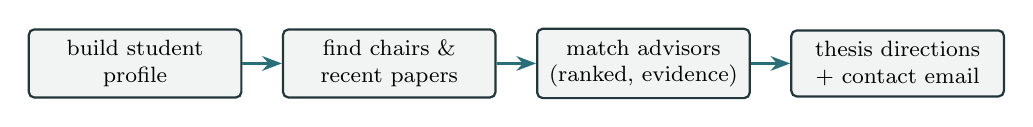
\begin{tikzpicture}[
      stage/.style={draw=sosDark, thick, rounded corners=2pt, fill=sosDark!6,
        align=center, font=\footnotesize, inner sep=4pt, minimum width=27mm},
      arr/.style={-{Stealth[length=2.5mm]}, thick, sosAccent}]
    \node[stage] (a) {build student\\profile};
    \node[stage, right=5mm of a] (b) {find chairs \&\\recent papers};
    \node[stage, right=5mm of b] (c) {match advisors\\(ranked, evidence)};
    \node[stage, right=5mm of c] (d) {thesis directions\\+ contact email};
    \draw[arr] (a) -- (b);
    \draw[arr] (b) -- (c);
    \draw[arr] (c) -- (d);
  \end{tikzpicture}
  \end{center}
  \vspace{0.5em}
  \begin{itemize}
    \item Input can be as thin as \emph{``I like deep learning and robotics''}
      --- the agent interviews the student to fill the gaps
    \item Every recommendation cites its evidence: papers, people, group pages
    \item The output coaches students toward a \emph{conversation} with the
      chair, not topic shopping
  \end{itemize}
\end{frame}

\begin{frame}{The data layer: a curated, public researcher tree}
  \begin{columns}[T]
    \begin{column}{0.46\textwidth}
      \begin{center}
      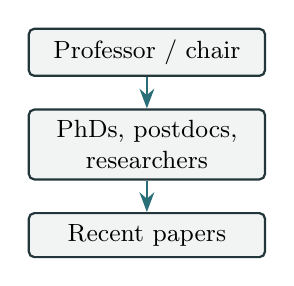
\begin{tikzpicture}[
          node distance=4mm,
          n/.style={draw=sosDark, thick, rounded corners=2pt, fill=sosDark!6,
            font=\small, inner sep=4pt, minimum width=30mm, align=center},
          arr/.style={-{Stealth[length=2.5mm]}, thick, sosAccent}]
        \node[n] (p) {Professor / chair};
        \node[n, below=of p] (r) {PhDs, postdocs,\\researchers};
        \node[n, below=of r] (w) {Recent papers};
        \draw[arr] (p) -- (r);
        \draw[arr] (r) -- (w);
      \end{tikzpicture}
      \end{center}
    \end{column}
    \begin{column}{0.52\textwidth}
      \small
      \begin{itemize}
        \item Built only from \textbf{already-public} sources: OpenAlex,
          publication records, official team pages
        \item Stored as plain, reviewable Markdown --- every entry carries
          provenance, dates, and uncertainty flags
        \item Refreshed by an automated monthly job as a reviewable change
          request; manual corrections are never silently overwritten
        \item Validated against hand-verified ground truth for pilot chairs,
          then scaled to all 47 professors
      \end{itemize}
    \end{column}
  \end{columns}
\end{frame}

\begin{frame}{How this answers the concerns you raised}
  \renewcommand{\arraystretch}{1.35}
  \small
  \begin{tabular}{@{}p{0.44\textwidth}p{0.5\textwidth}@{}}
    \toprule
    \textbf{You told us\ldots} & \textbf{So we\ldots} \\
    \midrule
    ``Don't build a system we have to use'' & built a student tool; chairs do nothing by default \\
    ``Read our existing websites instead'' & ingest public pages and publications --- no data entry \\
    ``Topics are co-created, not browsed'' & surface \emph{research areas and people}, and coach students toward conversation \\
    ``Too many misdirected inquiries'' & better-matched, better-prepared students $\Rightarrow$ fewer cold, low-signal emails \\
    ``Will it still exist in 3 years?'' & no chair investment to lose; your websites remain the source of truth \\
    \bottomrule
  \end{tabular}
\end{frame}

\begin{frame}{Privacy and governance}
  \begin{itemize}
    \item \textbf{Student data never leaves the session.} The profile
      (interests, transcripts, constraints) exists only in the student's own
      agent conversation --- nothing is stored or transmitted by us.
    \item \textbf{Only public academic data is bundled}: names, roles,
      publications, and research areas as published by chairs and OpenAlex.
      We document this policy explicitly with GDPR in mind.
    \item \textbf{Everything is inspectable.} Data and skills are plain text
      in a public repository; any chair can review --- or ask to correct ---
      what is said about their group.
    \item \textbf{No fabricated numbers.} A hard project rule: no placeholder
      metrics, no invented team sizes or citation counts.
  \end{itemize}
\end{frame}

\begin{frame}{Where we are, and what happens next}
  \textbf{Now --- Phase 1: get the data right first}
  \begin{itemize}
    \item Pipeline piloted on 3 chairs with hand-verified rosters as ground truth
    \item Gate before anything else: $\geq$\,90\% recall on pilot rosters,
      full referential integrity, reproducible golden record
  \end{itemize}
  \smallskip
  \textbf{Then --- Phase 2: optimize the advising behavior}
  \begin{itemize}
    \item Scale the researcher tree to all 47 professors
    \item Systematic evaluations: shallow profiles, missing information,
      degree-program and thesis-scope constraints (B.Sc.\ vs.\ M.Sc.)
  \end{itemize}
  \smallskip
  \textbf{Ordering principle:} matching cannot be trusted while the underlying
  data are incomplete or stale --- so data quality is gated before behavior
  tuning.
\end{frame}

\begin{frame}{What we ask of you (very little)}
  \begin{enumerate}
    \item \textbf{Nothing, by default.} The tool works from your public pages
      and publications as they are.
    \item \textbf{Optionally:} a handful of research-area keywords --- data
      that rarely needs revision. No logins, no dashboards, and a hard rule of
      \alert{no reminder emails}.
    \item \textbf{Feedback:} if inquiries you receive start arriving
      better-prepared, we would like to hear it --- that is our success metric,
      not platform adoption.
  \end{enumerate}
  \vspace{1em}
  \begin{center}
    \alert{Students get better discovery. You get fewer but better inquiries.\\
    Nobody is forced to maintain anything.}
  \end{center}
\end{frame}

\begin{frame}[standout]
  Thank you --- questions?
\end{frame}

\end{document}
